% !TEX program = xelatex

\documentclass[hidelinks, 12pt, a4paper]{article}

\usepackage{fontspec}
\setmainfont[Ligatures=TeX]{Linux Libertine O}

\usepackage[hidelinks, colorlinks = true, urlcolor = blue]{hyperref}

\usepackage{indentfirst}
\usepackage{graphicx}
\usepackage[left=2cm,right=2cm,top=2.5cm,bottom=2.5cm]{geometry}
\usepackage{lipsum}

%\setlength{\parindent}{1em}
%\setlength{\parskip}{1em}\title{Εργασία Στατιστικής}

%\title{Java socket programming \\ 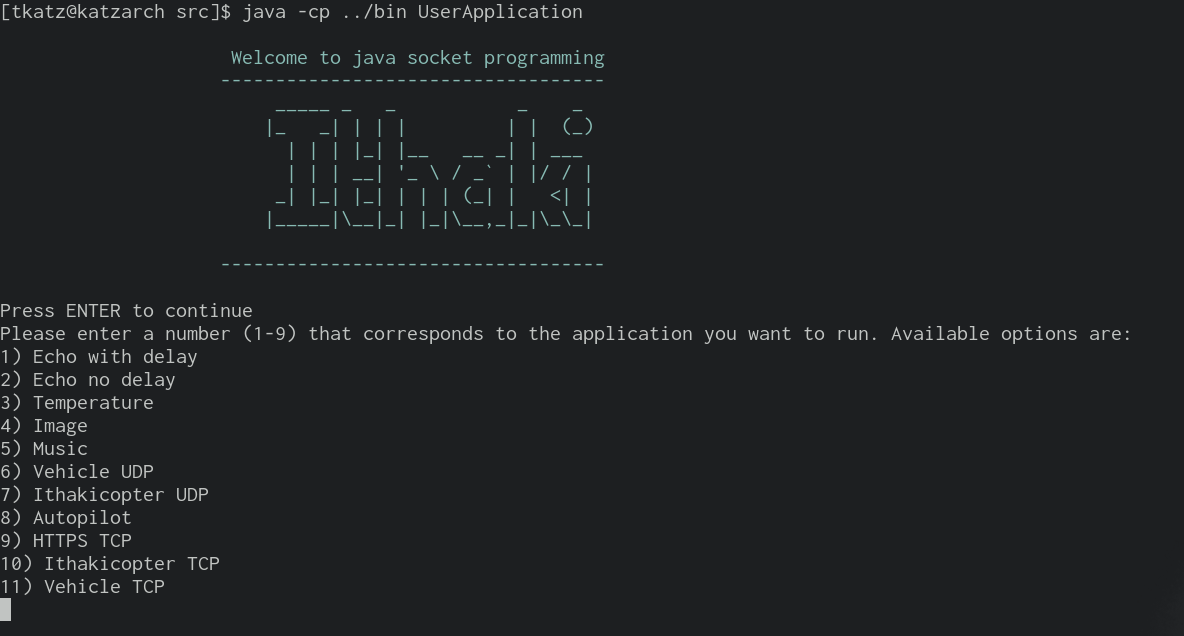
\includegraphics[width=\textwidth]{assets/login.png}}
% \author{Θεόδωρος Κατζάλης \\ ΑΕΜ:9282 \\ katzalis@auth.gr}
% \date{19/07/2020}

\begin{document}

\begin{titlepage}

\begin{figure}[h!]
  \begin{center}
    
\includegraphics[width=3cm]{assets/auth.pdf}
    \label{fig:cover_auth_logo}
  \end{center}
\end{figure}

\centering
\Large Αριστοτέλειο Πανεπιστήμιο Θεσσαλονίκης\\
\Large Πολυτεχνική Σχολή\\
%\large Τμήμα Ηλεκτρολόγων Μηχανικών και Μηχανικών Υπολογιστών\\
%\large Τομέας Τηλεπικοινωνιών

\vspace{\fill}

\LARGE \textbf{Java socket programming} \\
\LARGE \textbf{Δίκτυα 2}

\vspace{\fill}

\Large Θεόδωρος Κατζάλης \\
\Large ΑΕΜ:9282 \\ 
\Large katzalis@auth.gr

\vspace{\fill}
\raggedright

\centering
\vspace{\fill}
\today

\end{titlepage}

%\maketitle


\pagebreak
\tableofcontents
\pagebreak

% \section{Lorem}
% \lipsum


\section{G1}

\begin{figure}[h!]
\centering
	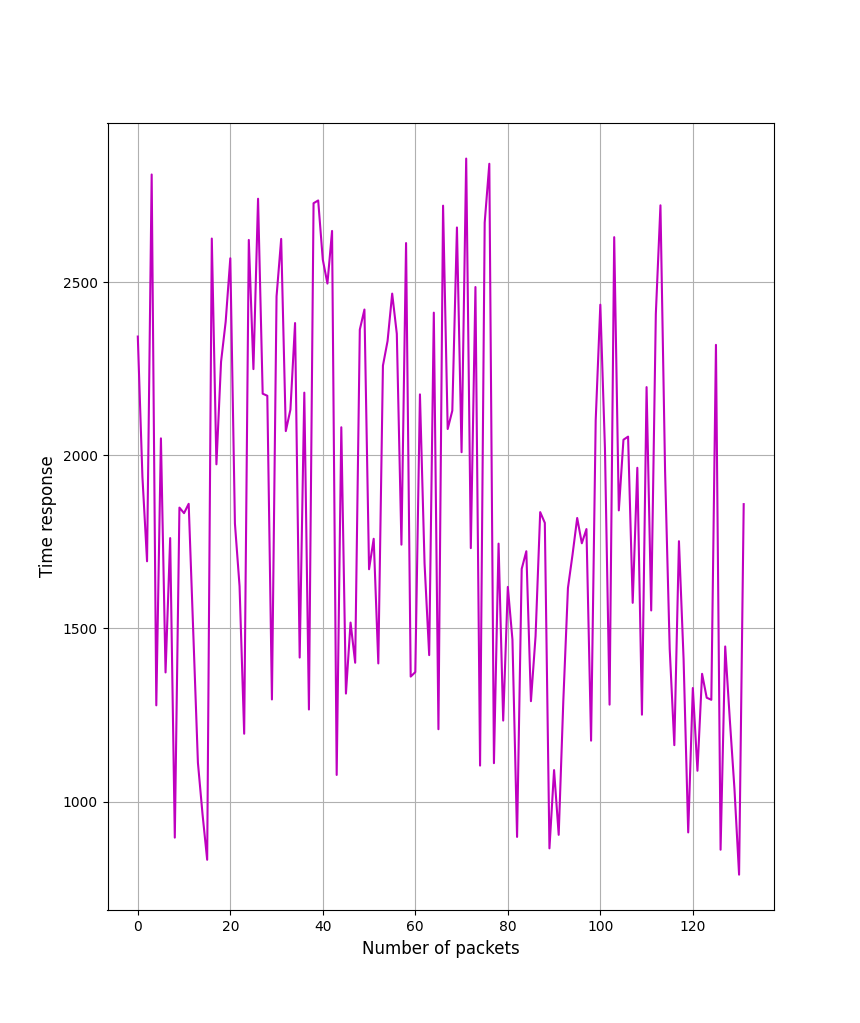
\includegraphics[height=.5\textheight, width=\textwidth]{assets/session1/g1.png}
	\caption{G1} 
\end{figure}

\section{G2}

\begin{figure}[h!]
\centering
	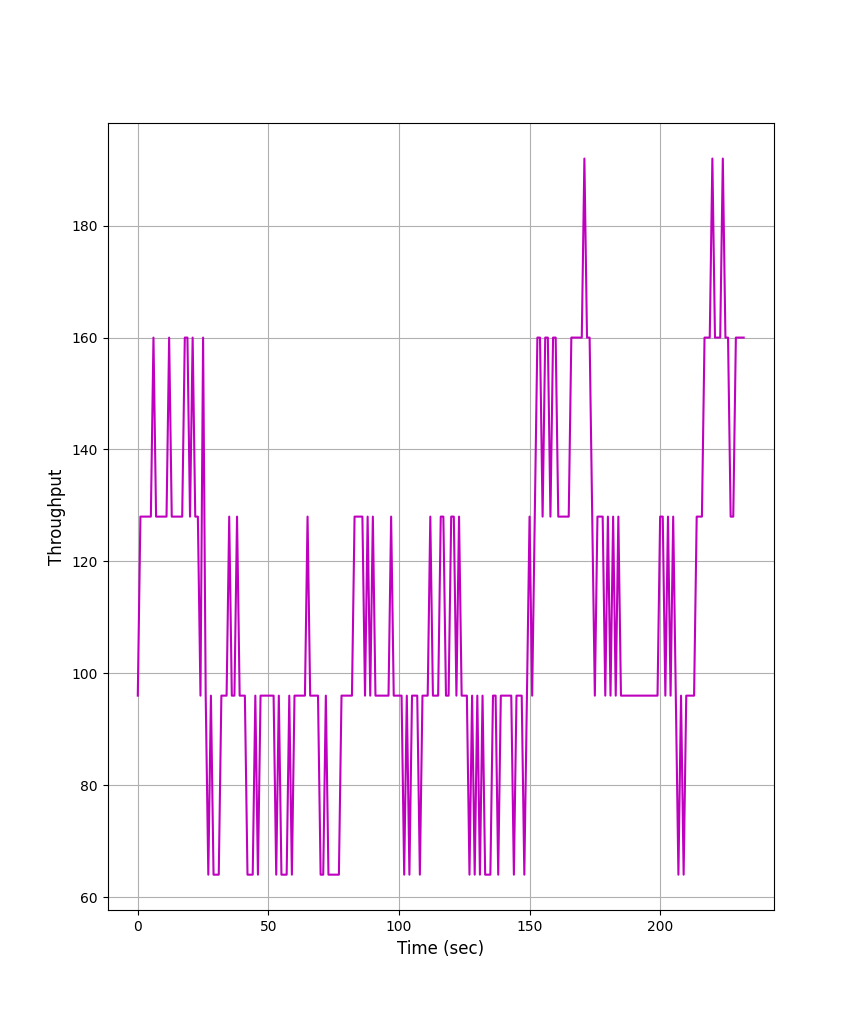
\includegraphics[height=.4\textheight, width=\textwidth]{assets/session1/g2.png}
	\caption{G2} 
\end{figure}

\section{G3}

\begin{figure}[h!]
\centering
	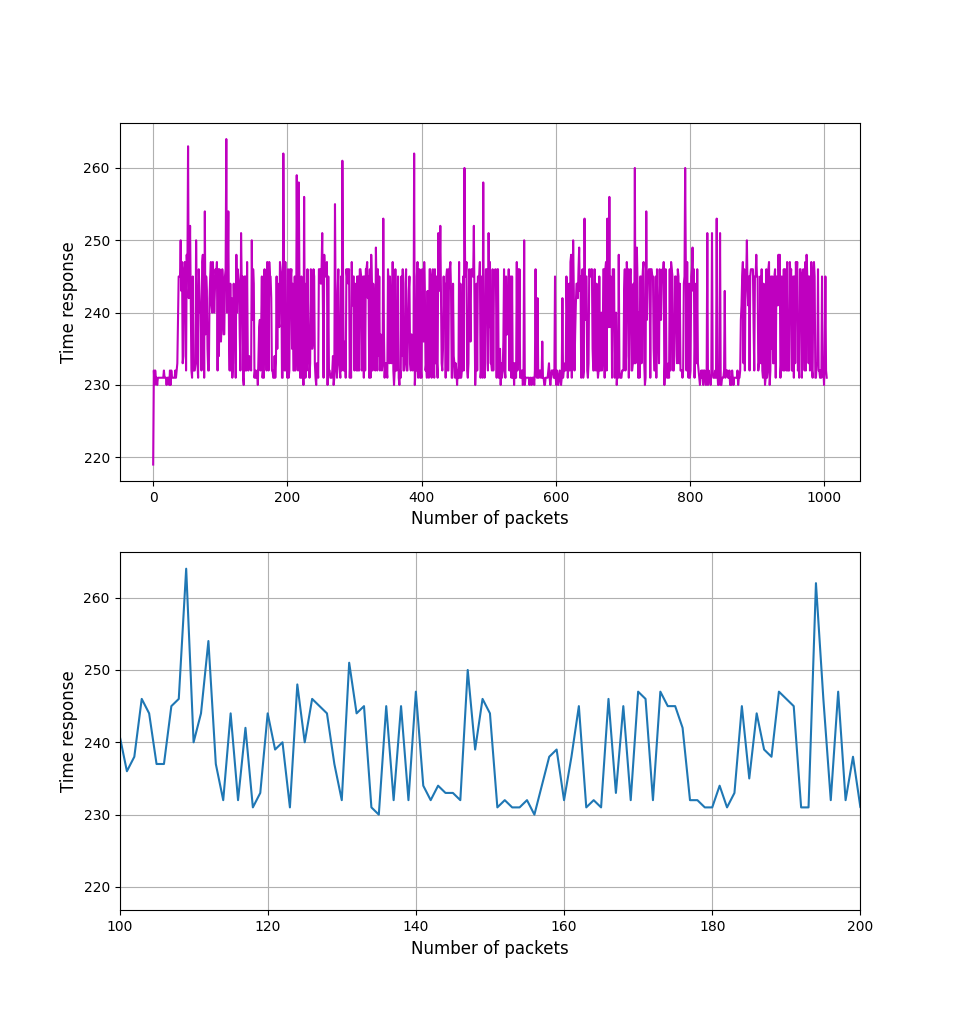
\includegraphics[height=.4\textheight, width=\textwidth]{assets/session1/g3.png}
	\caption{G3} 
\end{figure}

\section{G4}

\begin{figure}[h!]
\centering
	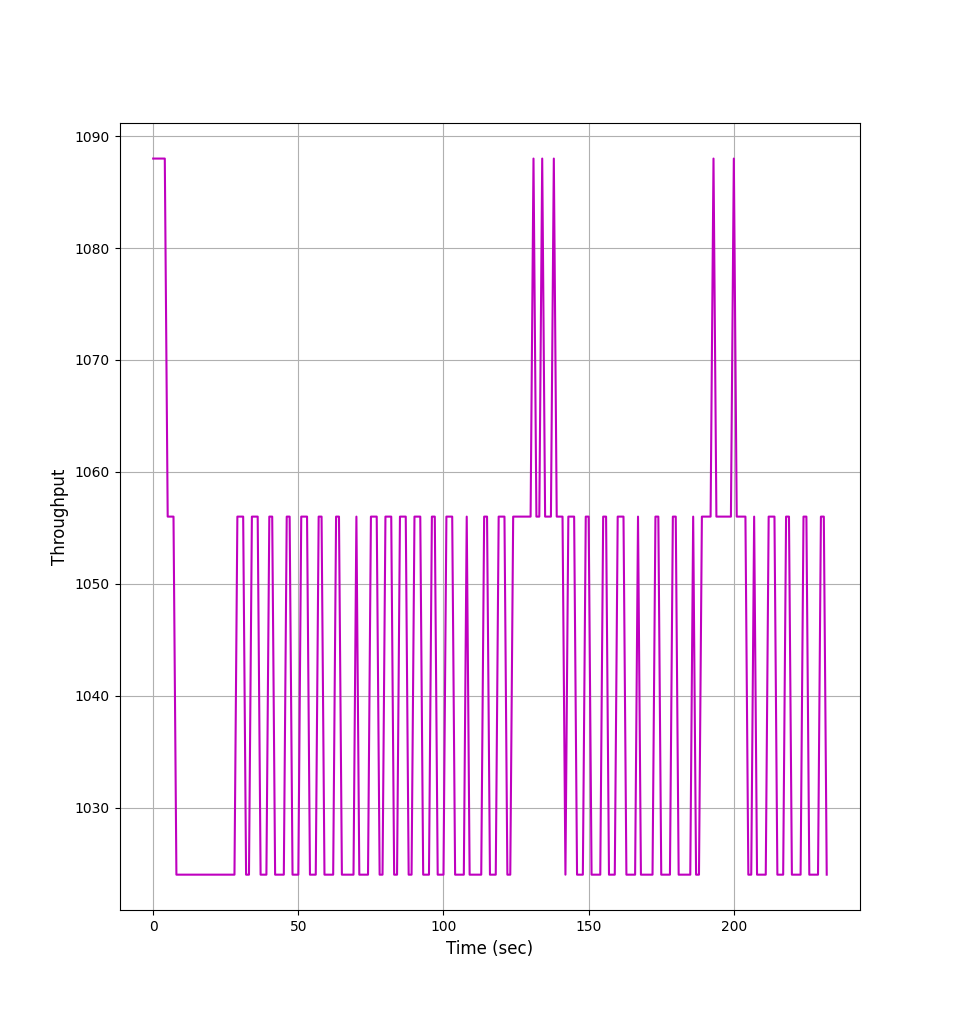
\includegraphics[height=.4\textheight, width=\textwidth]{assets/session1/g4.png}
	\caption{G4} 
\end{figure}

\section{G5}

\section{G6}

\section{G7}

\section{G8}

\section{R1}

\begin{figure}[h!]
\centering
	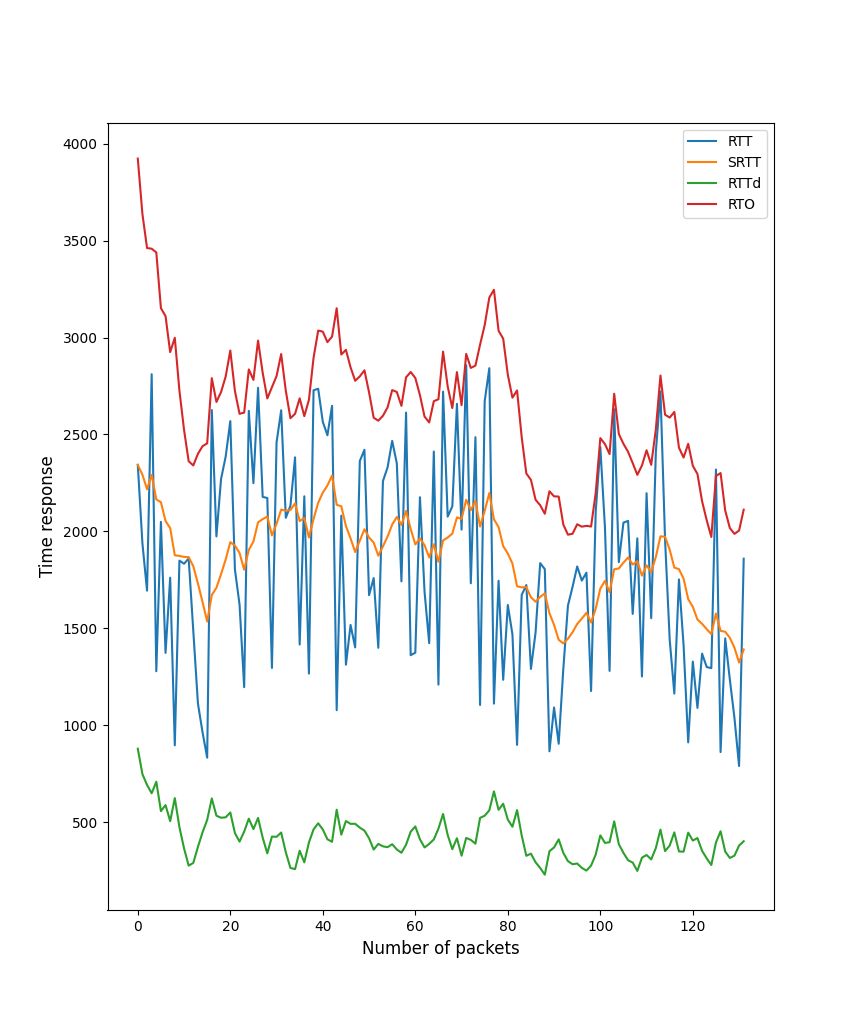
\includegraphics[height=.4\textheight, width=\textwidth]{assets/session1/r1.png}
	\caption{Retransmission timeout} 
\end{figure}

\section{E1}

\begin{figure}[h!]
\centering
	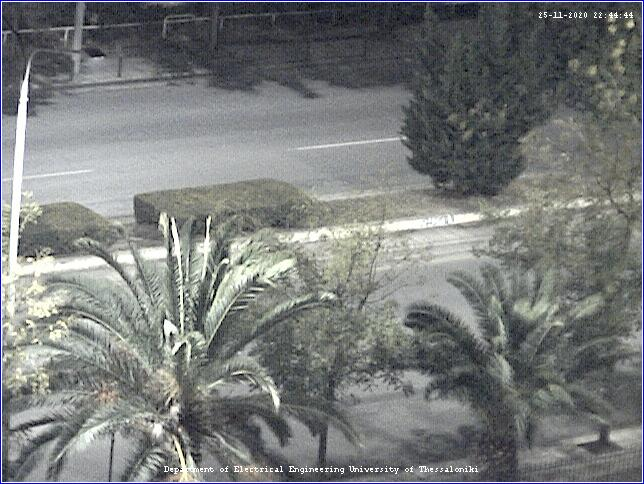
\includegraphics[height=.4\textheight, width=\textwidth]{assets/session1/image_fix.jpg}
	\caption{G4} 
\end{figure}

\section{E2}

\begin{figure}[h!]
\centering
	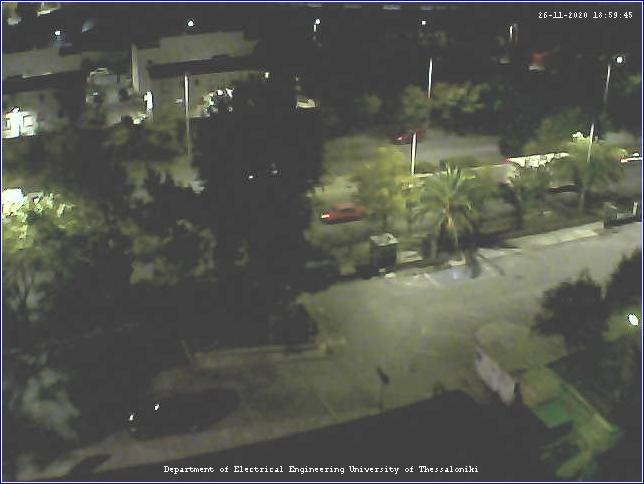
\includegraphics[height=.4\textheight, width=\textwidth]{assets/session1/image_ptz.jpg}
	\caption{Image PTZ} 
\end{figure}

\section{Temperature}



\section{G9}

\begin{figure}[h!]
\centering
	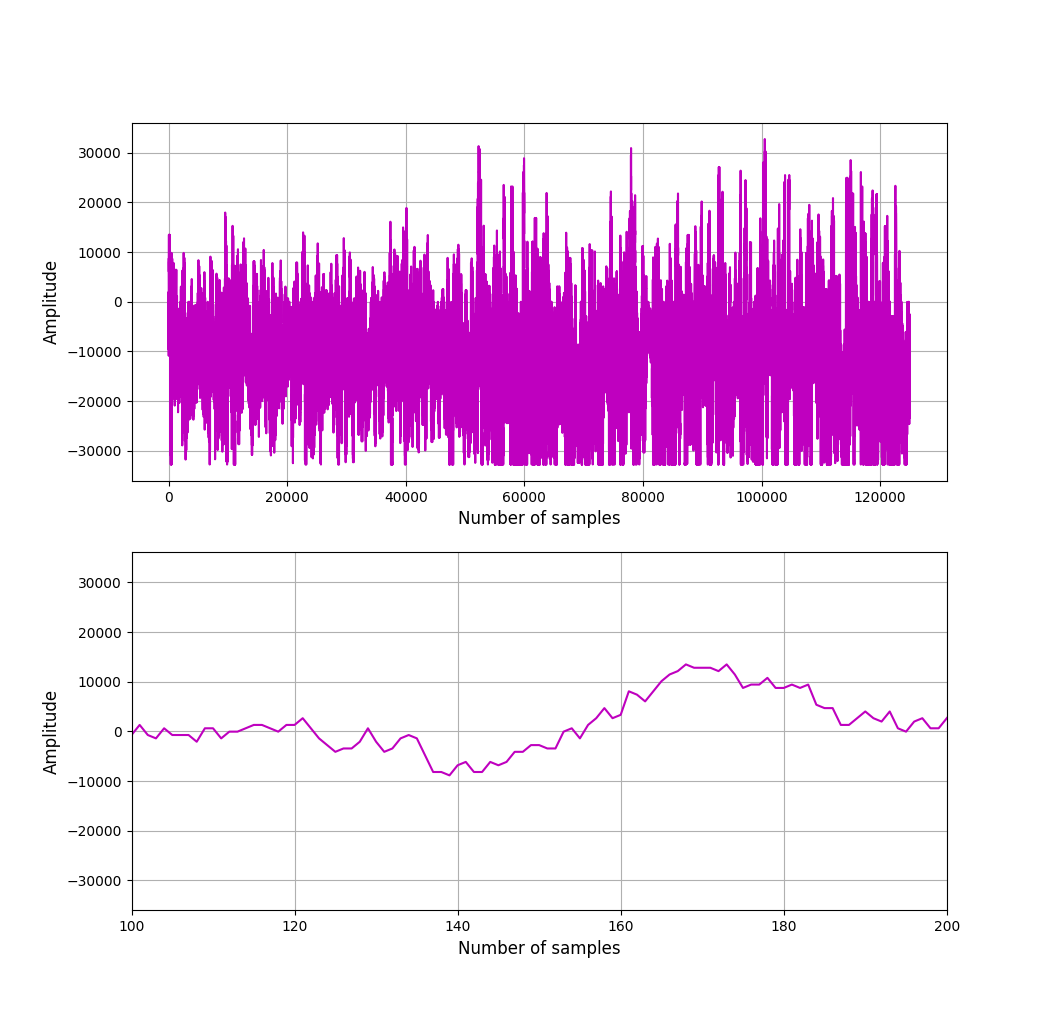
\includegraphics[height=.4\textheight, width=\textwidth]{assets/session1/g9_aq.png}
	\caption{AQDPCM samples waveform} 
\end{figure}

To find the time you need to check the wireshark!! We can see also the clipping effect!! Perfect!

\section{G10}

\begin{figure}[h!]
\centering
	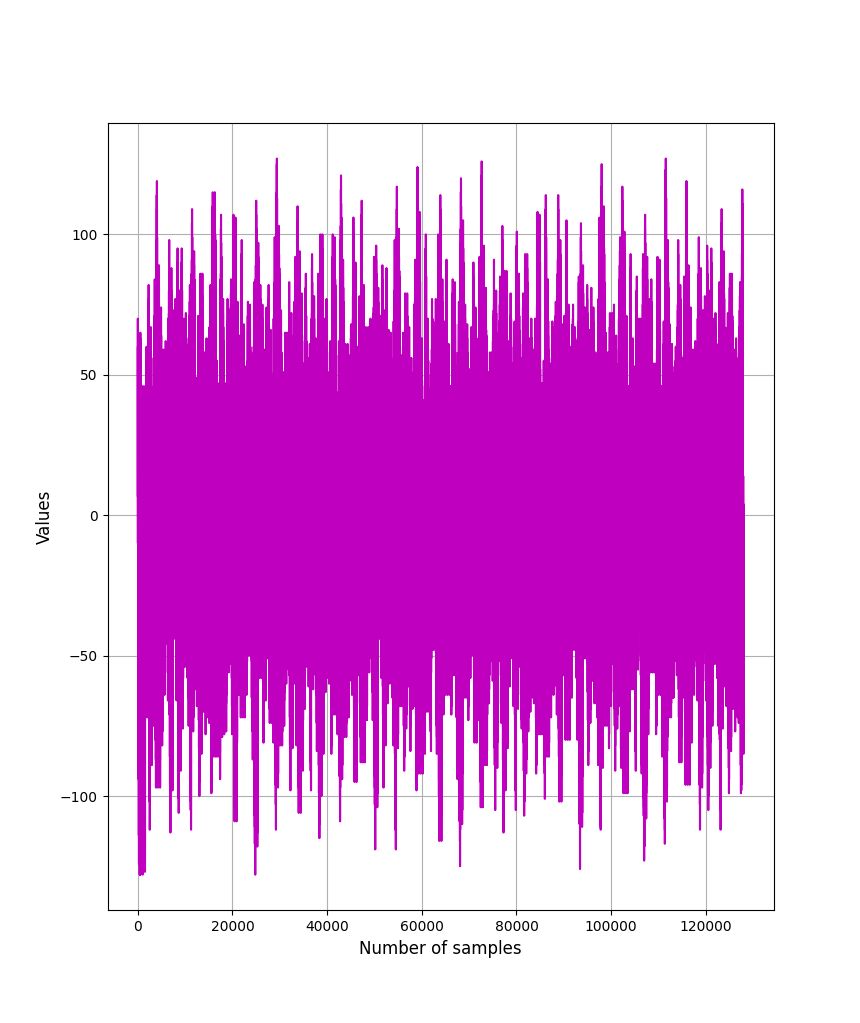
\includegraphics[height=.4\textheight, width=\textwidth]{assets/session1/g10.png}
	\caption{DPCM samples waveform Tone} 
\end{figure}

The file to find the time is the Tmusic\_info.txt. We can also see the clipping effect!

\section{G15}

\begin{figure}[h!]
\centering
	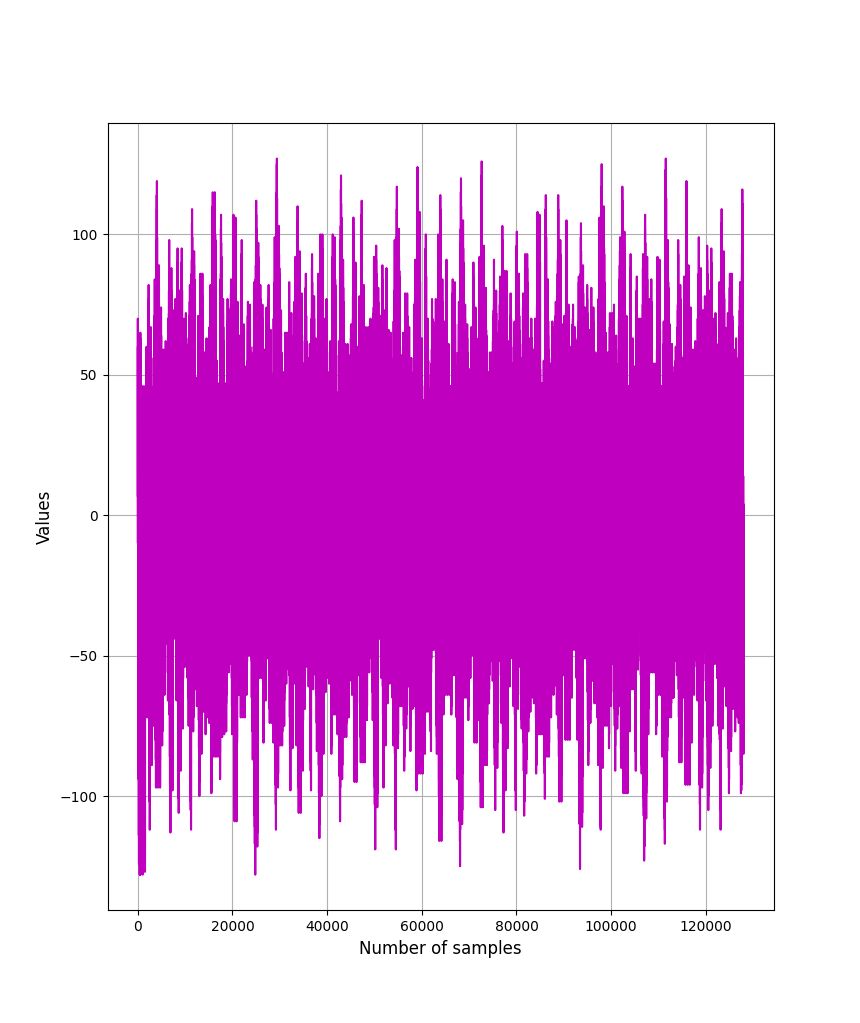
\includegraphics[height=.4\textheight, width=\textwidth]{assets/session1/g10.png}
	\caption{Mean 1st clip} 
\end{figure}

\section{G16}

\begin{figure}[h!]
\centering
	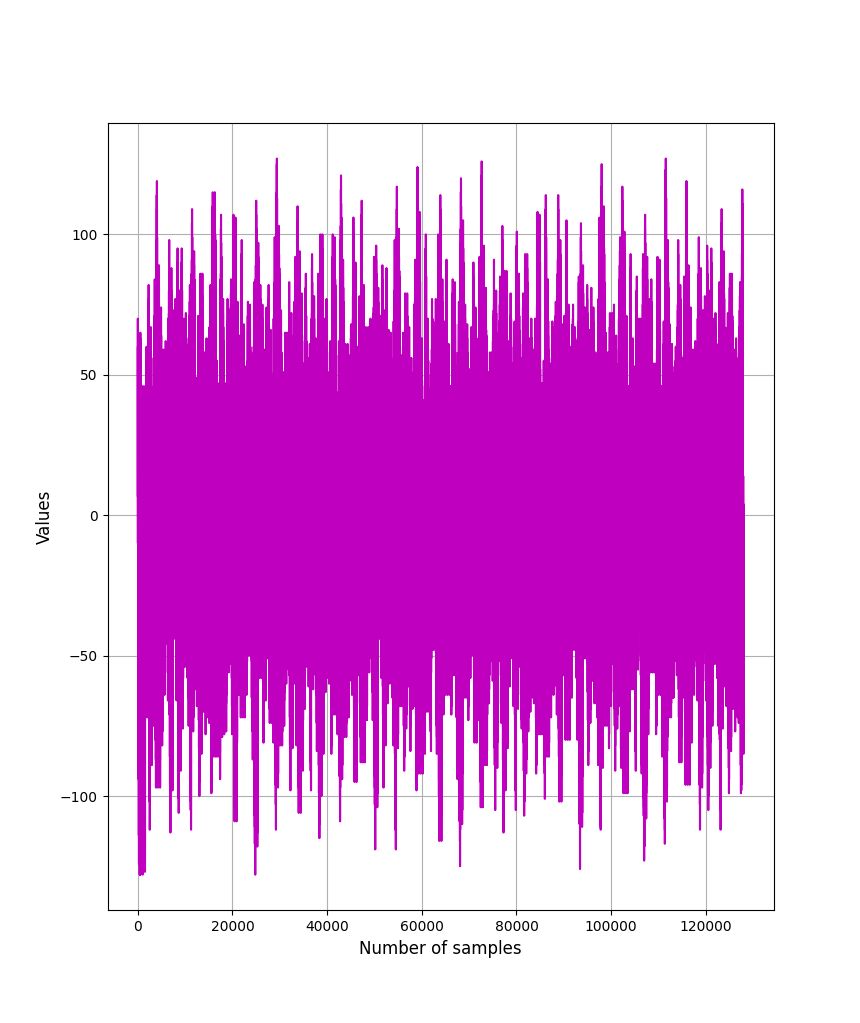
\includegraphics[height=.4\textheight, width=\textwidth]{assets/session1/g10.png}
	\caption{Mean 1st clip} 
\end{figure}

\end{document}
